%% logical setup, no need to edit %%%%%%%%%%
\newif\ifboyscout                         %%
\boyscouttrue %% commented, WWW/boyscouts %%
\newif\ifpreparepdf                       %%
\preparepdftrue % hyperlinked pdf default %%

\newif\ifbackground % whether use background image
\backgroundfalse
\newif\iflogo % whether use logo
\logotrue
\newif\ifpsd % whether include psd.tex
\psdfalse
\newif\ifnotes % whether show notes.
\notesfalse
\newif\ifhandout % handout mode
\handoutfalse
\newif\ifwetwild % whether for wet&wild or SIAM student
\wetwildfalse

\ifhandout
\documentclass[mathserif, handout]{beamer}
\else
\documentclass[mathserif]{beamer}
\fi

\usepackage{graphicx}
%\usepackage{tabu}
\usepackage{algpseudocode}
\usepackage{algorithm}
\usepackage{tikz}
\usetikzlibrary{calc}
\usetikzlibrary{decorations.pathreplacing}
\usepackage{tipa}
\usepackage{movie15}
\input ../defsSchur
\input ./defChaosBook

\graphicspath{{../../xiong/figures/}{./figs/}}



% ------                       setup of beamer               ----------------
\usetheme{Madrid}

\ifnotes
\setbeameroption{show notes}
\else
\setbeameroption{hide notes}
\fi

\setbeamertemplate{bibliography item}[text]
%  add background image
\ifbackground
\usebackgroundtemplate
{
  
\includegraphics[width=\paperwidth,height=\paperheight]{./figs/background.jpg}%
}
\fi

% -------------------      title page       --------------------------
\title[Periodic eigendecomposition] % (optional, only for long titles)
{Periodic Eigendecomposition}
\subtitle{and its application in nonlinear dynamics}
\logo{
  \iflogo
  
\includegraphics[width=2cm,height=1cm,keepaspectratio]{./figs/gtlogo}
  
\includegraphics[width=1cm,height=0.8cm,keepaspectratio]{./figs/cnslogo}
  \fi
}
\author[Xiong, Predrag] % (optional, for multiple authors)
{Xiong Ding %\inst{1}
    and
Predrag Cvitanovi\'c%\inst{1}
}
\institute[Gatech] % (optional)
{
  %\inst{1}%
  School of Physics\\
  Georgia Institute of Technology
}
\ifwetwild
\date[Wet\&wild 2014] % (optional)
{Wet\&wild discussion group, 2014}
\else
\date[SIAM student 2014] % (optional)
{Georgia Tech SIAM Student Chapter Seminar \\ October 17, 2014}
\fi

\subject{Computer Science}

%  ----------------    setup of outline    -------------------------
\iffalse
\AtBeginSection[]
{
  \begin{frame}
    \frametitle{Table of Contents}
    \tableofcontents[currentsection]
  \end{frame}
}
\fi

\AtBeginSubsection[]
{
  \begin{frame}
    \frametitle{Table of Contents}
    \tableofcontents[currentsection,currentsubsection]
  \end{frame}
}

%  ---------------   main content of slides  -----------------------
\begin{document}
\frame{\titlepage} % add title page.

%  ----------------  section: definition of problem --------------

\section{Introduction}
\subsection{Physical background}
\begin{frame}
  \frametitle{example : R\"{o}ssler flow}
  \begin{figure}[h]
    \centering
    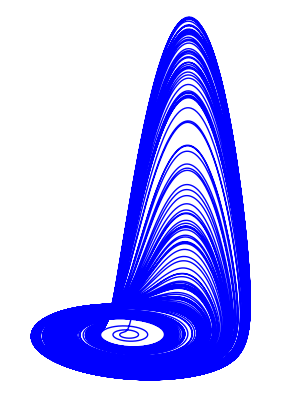
\includegraphics[width=0.25\textwidth]{ergodic} %\hfill
    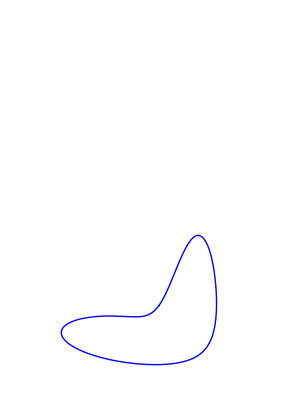
\includegraphics[width=0.25\textwidth]{po1} %\hfill
    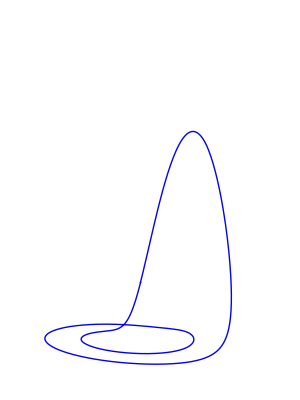
\includegraphics[width=0.25\textwidth]{po2} %\hfill
    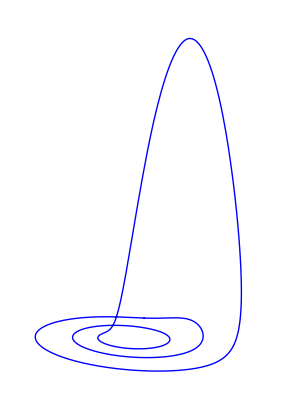
\includegraphics[width=0.25\textwidth]{po3} %\hfill
  \end{figure}

\bea
    \dot{x} &=&  -y - z
    \continue
    \dot{y} &=&  x +ay
    \continue
    \dot{z} &=&  b +z(x-c)\,, \quad a=b=0.2 \,,\; c=5.7
    %\,.
\nnu
\eea

\end{frame}

\begin{frame}
  \frametitle{Cycle expansions}
  {\color{cyan} Ergodic averages} are given by eigenvalues of
  the spectral determinant, which can be evaluated
  from a sum over of periodic orbits~\cite{DasBuch}
  \[
  \det(1-z\Lop) =  \exp \left(
    \sum_{p} \sum_{r=1}^\infty \frac{1}{r}
    \frac{  z^{\cl{p} r }  e^{r \beta \cdot  \Obser_{p}} }{\oneMinJ{r}}
  \right)
  \]
\[
\det (M_p) = \prod \Lambda_i \,,\quad \Lambda_i
    \mbox{: eigenvalues of Jacobian matrix} J_p
\]
  \[
  J_p = J(x_n)J(x_{n-1})\cdots J(x_1), \quad x_n =x_1
  \]

  \begin{columns}[c]
    \column{0.5\textwidth}
    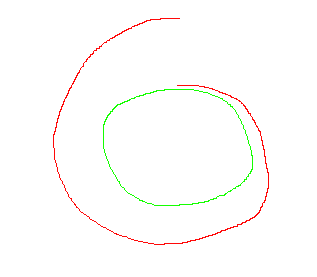
\includegraphics[width=0.5\textwidth]{./figs/p1}
    \column{0.5\textwidth}
    $\delta x(\period{p}) = J_p\delta x(0) $
  \end{columns}

\end{frame}

\begin{frame}
  \frametitle{Dominated splitting}
  For an $f$-invariant set $\Lambda$, an invariant splitting
  \[
  T_\Lambda M = E \oplus F
  \]
  \[
  ||Df^{n}_{/E(x)}||\cdot||Df^{-n}_{/F(f^n(x))}|| \le C\lambda^n \,,\quad
  \text{for all} \quad x\in\Lambda\,, n\ge 0
  \]
  with $C>0$ and $0<\lambda<1$.

  \vspace{1.5em}
  \pause

  If $E$ is {\color{green} uniformly contracting} :

  Local dimensions of a chaotic attractor is expanded by
  a {\color{red} subset of covariant vectors}~\cite{ginelli-2007-99}.

  \note[item]<1>{
    I need to explain what $M_p^r$ is.
  }
  \note[item]<1>{
    Remember that for our case, $E(x)$ is the contracting subspace.
  }
\end{frame}

\subsection{Definition of the problem}

\begin{frame}
  \frametitle{Eigendecomposition}
  A product of $m$ real matrices
  \begin{equation}
    \ps{\jMps}{0}=\jMps_{m}\jMps_{m-1}\cdots \jMps_{1}\,,\quad
    \jMps_{i}\in \mathbb{R}^{n\!\times\! n},\; i\!=\!1,2,\cdots,m
    \label{eq:problem}
  \end{equation}
  can be {\color{red} diagonalized}
  \textbf{iff} the sum of dimensions of eigenspaces of
  $\ps{\jMps}{0}$ is $n$.
  \begin{equation}
    \label{eq:diagonal}
    \ps{\jMps}{0}=V^{(0)}D(V^{(0)})^{-1}
    \,,
  \end{equation}

  \begin{center}
    $D = \text{diag}(\ExpaEig_{1},\ExpaEig_{2},\cdots,\ExpaEig_{n})$,
    $V^{(0)}=[v^{(0)}_{1},v^{(0)}_{2},\cdots,v^{(0)}_{n}]$.
  \end{center}

  \begin{block}{Floquet vectors and Floquet exponents}
    \[
    J_p(x)e_i(x)=e^{\lambda_i T_p}e_i(x)\,,
    \quad \lambda_i = \mu_i + i\omega_i
    \]
  \end{block}

  \note[item]<1>{
    Explain the definition of Floquet exponents/vectors:
    \begin{itemize}
    \item subscript p means that the Jacobian is evaluated\\
      along a  periodic orbit.
    \item $\mu$ characterizes the expanding rate. $\omega$ characterize\\
      the rotating velocity for complex vectors.
    \end{itemize}
  }


  \note[item]<1>{
      where $D$ is a diagonal matrix which stores $\ps{\jMps}{0}$'s
      eigenvalues, $\{ \ExpaEig_{1},\ExpaEig_{2},\cdots,\ExpaEig_{n}\}$.

      Columns of matrix $V^{(0)}$ are the eigenvectors of $\ps{\jMps}{0}$:
      $V^{(0)}=[v^{(0)}_{1},v^{(0)}_{2},\cdots,v^{(0)}_{n}]$.
    }
\end{frame}

\begin{frame}
  \frametitle{Challenges}
  Two main challenges:
  \begin{itemize}
  \item
    {\color{green} Overflow\quad\&\quad Underflow} \\

    They should not be multiplied up into a single matrix.

    \vspace{1em}
    \pause

  \item
    {\color{green} Cyclic rotations}

    \[
    \ps{\jMps}{k}=\jMps_{k}\jMps_{k-1}\cdots \jMps_{1}\jMps_{m}\cdots
    \jMps_{k+1} \quad \text{for}\quad k=1,2,\dots,m\!-\!1
    \]
    $\ps{\jMps}{0}$ vs $\ps{\jMps}{k}$ :
    \begin{itemize}
      \normalsize{
    \item same eigenvalues.
    \item eigenvectors are related by $\jMps_{m}\cdots\jMps_{k+1}$
      }
    \end{itemize}

    \vspace{1em}
    \pause

    {\color{red} Pitfall}:
    noise is accumulating in the matrix multiplication process.

  \end{itemize}

  \note[item]<1>{
    Eigendecomposition of the cyclic rotations is also desired.
  }

\end{frame}

\subsection{Covariant vectors algorithm}

\begin{frame}
  \frametitle{We all like him:}
  \begin{columns}[c]
    \column{0.45\textwidth}
    \begin{figure}[h]
      \centering
      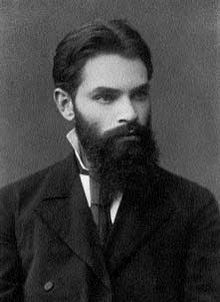
\includegraphics[width=1.0\textwidth]{Alexander_Ljapunow_jung}
    \end{figure}

    \pause

    \column{0.35\textwidth}
    \textbf {\large{ Aleksandr Lyapunov}}
 \end{columns}

  \note[item]<1>{
    We all like this guy. There are exponent, equation, function
    named after him. Even some kind of dimension is named after him.
  }
\end{frame}

\begin{frame}
  \frametitle{Oseledets splitting~\cite{ruelle79}}
  Dynamics in tangent space : $J^n(x)=\partial f^n(x)/\partial x$.
  \begin{itemize}
  \item $\Lambda^{\pm}(x) :=\lim_{n\to\pm\infty}[J^n(x)^\top J^{n}(x)]^{1/2n}$
    exist.

  \item eigenvalues are
    \[
    e^{\lambda^{\pm}_1(x)}<\cdots<e^{\lambda^{\pm}_s(x)}
    \,.
    \]
    $\lambda^{+}_i(x)=-\lambda^{-}_{s-i+1}(x)=\lambda_i$ are
    \textbf{Lyapunov exponents}.
    The corresponding eigenspaces:
    \[U^\pm_1(x), \cdots, U^\pm_s(x)\]

    \pause
  \item
    $
    V^+_i(x)=U^+_1(x)+\cdots+U^+_i(x),\quad
    V^-_i(x)=U^-_s(x)+\cdots+U^-_{s-i+1}
    $
    Then
    {\color{green} $W_i(x)=V^+_i(x)\cap V^-_i(x)$} is
    dynamically {\color{red} forward}
    and {\color{red} backward} invariant:
    {\color{green}
      \[J^{\pm n}(x)W_i(x) \to W_i(f^{\pm n}(x))\].
    }
  \end{itemize}

  \note[item]<1> {
    Before diving into the details of this algorithm directly,
    let me first introduce what covariant vectors refer to.  Physicists
    and mathematicians use different terminologies, so I am 100 percent
    sure all of you know this.
  }
  \note[item]<1>{
    \[U^\pm_1(x), \cdots, U^\pm_s(x)\] are not flow invariant.
  }
  \note[item]<1>{
    Mention this :
    \[
    \lim_{n\to\pm\infty}\frac{1}{|n|}\ln||J^n(x)u|| =
    \pm\lambda_i\quad\text{when}\quad
    u\in W_i(x)
    \]
  }
  \note[item]<1>{
    How to say: V plus is the union of the first $i$ eigenspaces
    of matrix Lambda plus.}
  \note[item]<1>{
    How to calculate $W_i(x)$ numerically?
  }

  \note[item]<1>{
    multiplicative ergodic theorem.
  }
\end{frame}



\begin{frame}
  \frametitle{Covariant vectors algorithm~\cite{GiChLiPo12}}

  \input figCLV.tex

  $W_i(x)$ reduce to \textbf{Floquet vectors} for periodic orbits.


  \pause

  {\color{green} Limitations of this algorithm:}
  \begin{itemize}
  \item cannot distinguish complex conjugate pairs
  \item low efficiency, especially when Floquet exponents cluster
  \end{itemize}



  \note[item]<1>{
    \textbf{Covariant vectors algorithm}: calculate $W_i(x)$ for an ergodic
    trajectory.
  }
\end{frame}



\subsection{Periodic Schur decomposition}

\begin{frame}
  \frametitle{Periodic Schur decomposition%
~\cite{Bojanczyk92theperiodic}}
\textbf{periodic real Schur form (PRSF)}.
  \begin{equation}
    \label{eq:prsf}
    \jMps_{i}=Q_{i}R_{i}Q_{i-1}^\top
    \,,
  \end{equation}
\begin{equation}
  \label{eq:pedrotation}
  \ps{\jMps}{k}=Q_{k}\ps{R}{k}Q_{k}^\top
  \,,
\end{equation}
with
$\ps{R}{k}=R_{k}R_{k-1}\cdots R_{1}R_{m}\cdots R_{k+1}$. Here, $R_i$ are
{\color{red} upper-triangular} matrices except that $R_m$ is
{\color{red} quasi-upper-triangular}.
$Q_i$ are orthogonal matrices.

\pause

\begin{columns}[c]
  \column{0.5\textwidth}
  Two stages:
  \begin{itemize}
  \item Hessenberg-triangular form
  \item Iteration of periodic QR algorithm
  \end{itemize}

  \column{0.5\textwidth}
  \begin{figure}[h]
    \centering
    
\includegraphics[width=0.6\textwidth]{per_schur_algorithm.pdf}
  \end{figure}

\end{columns}


  \note[item]<1>{If the audience asks about the details, then tell
    them that they are already documented in literature and is
    not the focus of this talk.}

\end{frame}

\ifpsd
\input psd
\fi
% -------      section: periodic eigendecomposition ----------
\section{periodic eigendecomposition}

\subsection{First stage: obtaining PRSF}

\begin{frame}
  \frametitle{Simultaneous iteration~\cite{Trefethen97}}
    If $\ps{\jMps}{0}$ has real, without degeneracy, eigenvalues
\[
|\ExpaEig_{1}|>|\ExpaEig_{2}|>\cdots >|\ExpaEig_{n}|
\,,
\] with
    corresponding normalized eigenvectors
\[v_{1},v_{2},\cdots ,v_{n}\]

    \begin{columns}

      \column{0.5\textwidth}
      \input figSI.tex

      \pause

      \column{0.5\textwidth}
      $q_{1}=v_{1}$,\quad  \pause
      $q_{2} = \frac{ v_{2}-(v_{2}^\top q_{1})q_{1} }{||\cdot||}$,

     \pause
     \vspace{1em}

      $q_{3} = \frac{ v_{3}-(v_{3}^\top q_{1})q_{1}-(v_{3}^\top q_{2})q_{2}}
      {||\cdot||}$

      \[
      [q_1, q_2, q_3] = [v_1, v_2, v_3]
      \begin{bmatrix}
        * & * & * \\
          & * & * \\
          &   & * \\
      \end{bmatrix}
      \]
    \end{columns}

    \pause
    {\color{green}
    \[
    q_{n} = \frac{v_{n}-\sum_{i=1}^{n-1}(v_{n}^\top q_{i})q_{i}}{||\cdot ||}
    \,.
    \]
  }

  \note[item]<1>{
    Two ways to obtain PRSF
    \begin{itemize}
    \item {\color{cyan} Periodic Schur decomposition} just introduced. \\
      Iteration of periodic QR algorithm (extended from Francis algorithm)

    \item {\color{cyan} simultaneous iteration}. \\
      Power iteration followed by QR decomposition
    \end{itemize}
  }

  \note[item]<1>{
    During the presentation, indicate that this is the main subject of this
    talk. Like ``Now we come to tackle the main problem we proposed
    at the beginning: how to get the eigenvectors...''
  }

\end{frame}


\begin{frame}
  \frametitle{ What if there are complex conjugate pairs?}
  \[
  \ps{\jMps}{0}Q_{0}=Q^{'}_{0}\ps{R}{0}=Q_{0}B\ps{R}{0}
  \,.
  \]
  $B$ is a {\color{red} block-diagonal} matrix with diagonal
  elements $\pm 1$
  or $[2\!\times\! 2]$ blocks.


  \note[item]<1>{
   $\pm 1$
   (corresponding to real eigenvalues).
   $[2\!\times\! 2]$ blocks (corresponding to complex eigenvalue pairs).
  }

\end{frame}

\subsection{Floquet exponents in  \KSe}

\begin{frame}
  \frametitle{\KSe~\cite{SCD07}}
  a flame on a ring, with the flame velocity satisfying
  \[
  u_t+\frac{1}{2}(u^2)_x+u_{xx}+u_{xxxx}=0\,,\quad x\in [0,L]
  \]
  In out simulations $L=22$.

  \begin{subequations}
    \bea
    \dot{a}_k  &=&
    ( q_k^2 - q_k^4 )\, a_k
    - i \frac{q_k}{2} \mathcal{F}[(\mathcal{F}^{-1}[a])^2]_k
    \,, \label{eq:ksfourier} \\
    \dot{a}_{N/2} &=&
    ( q_{N/2}^2 - q_{N/2}^4 )\, a_{N/2}
    \label{eq:highfourier}
    \,.
    \eea
  \end{subequations}

  \note[item]<1>{
    \textbf{Integrator} : Exponential time-differencing with 4th order
    Runge-Kutta.

    \textbf{Eigendecomposition}: \pqr\ \& reordering.
  }

  \pause

symmetries :
  \begin{itemize}
  \item {\color{cyan} Galilean invariance} :
    $u(x-ct,t)+c$ is also a solution,
    \\
    different by mean velocity $\int dx\, u$.
    {\color{red} Used} in the integrator.

  \item {\color{cyan} Reflection symmetry} :
  $Ru(x,t)=-u(-x,t)$ is also a solution.

  \item {\color{cyan} Transitional invariance} :
    $\tau_{l/L}u(x,t)=u(x+l,t)$.
  \end{itemize}

\end{frame}

\begin{frame}
  \frametitle{Benefit of symmtries}
  {\color{green} Benefit}:
  \begin{itemize}
  \item  Discrete symmetry $\Leftrightarrow$ dynamics reduced into
    fundamental domain.
  \item   Continuous symmetry $\Leftrightarrow$ \statesp\ dimension decreased by one.

  \item
    $
    \text{Continuous symmetry} \Leftrightarrow
    \text{marginal direction} \Leftrightarrow
    \text{group tangent}
    $
  \end{itemize}

  \pause

  \begin{exampleblock}{Two marginal directions ($|\ExpaEig_{i}|=1$) in the
      tangent space:}
  velocity field \quad \&\& \quad group tangent of transitional invariance.
  \end{exampleblock}

\end{frame}

\begin{frame}
  \frametitle{Example}
  \begin{figure}[h]
    \centering
    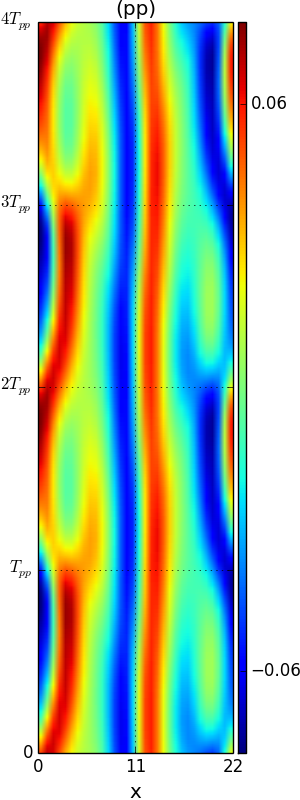
\includegraphics[width=0.255\textwidth]{KSppo1State}
    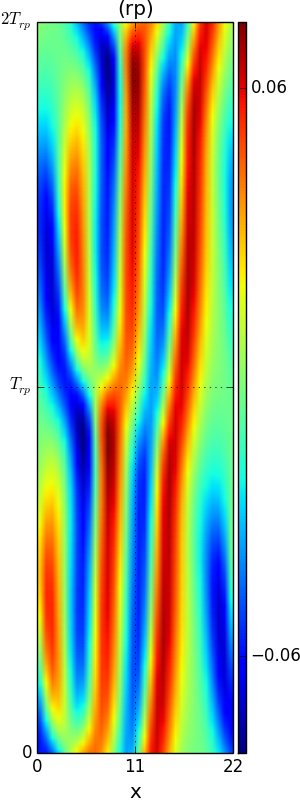
\includegraphics[width=0.255\textwidth]{KSrpo1State}
  \end{figure}
\end{frame}

\begin{frame}
  \frametitle{Floquet exponents}

  \begin{table}[h]
    \footnotesize
    \centering
    \caption{
      {\color{red} $ \ExpaEig_i= \exp(\period{}\,\eigRe[i] \pm i\theta_{i})$},
      for
      orbits $\cycle{pp}$ and $\cycle{rp}$, respectively.
      Truncation number $N=32$.
      {\color{green} $T_{pp} = 10.25$, $T_{rp} = 16.31$}.
    }
    \label{tab:floquet_ppo1}
    \begin{tabu}{l l c|[1pt]l l c}
      % \tabucline[1pt]{-}
      \multicolumn{3}{c|[1pt]}{$\cycle{pp}$} & \multicolumn{3}{c}{$\cycle{rp}$}\\
      $i$ & ~~~~~$\eigRe[i]$  & $\theta_{i}$  & $i$ & ~~~~~$\eigRe[i]$ & $\theta_{i}$  \\
      \tabucline[1pt]{-}
      1,2 & ~0.033209  &    $\pm$2.0079  &  1 &    ~0.32791  &              \\
      3 & -2.0317e-14  &                 &  2 &   ~5.0352e-09  &              \\
      4 & -2.4267e-09  &    -1           &  3 &  -1.2399e-08  &              \\
      5 &  -0.21637    &                 &  4 &     -0.13214  &        -1    \\
      6,7 &  -0.26524  &   $\pm$2.6205   &  5,6 &   -0.28597  & $\pm$2.7724  \\
      8 &  -0.33073    &    -1           &  7 &     -0.36242  &              \\
      9 &  -1.9605    &                  &  8 &      -0.32821  &      -1     \\
      10 & -1.9676    &    -1            &  9,10 &   -1.9617  &  $\pm$2.2411 \\
      $\cdots$ &  $\cdots$    & $\cdots$ & $\cdots$ & $\cdots$ & $\cdots$   \\
      27 &  -239.52   &                 & $\cdots$ & $\cdots$ &  $\cdots$   \\
      28 &  -239.22    &    -1           &  27,28 &    -239.41& $\pm$0.88159 \\
      29 & -307.47     &    -1           &  29 &      -313.98 &              \\
      30 & -332.74     &                 &  30 &      -323.41 &              \\
      \tabucline[1pt]{-}
    \end{tabu}
  \end{table}

  \note[item]<1>{
    point out: complex Floquet exponents, two marginal exponents, and
    large span.
  }
\end{frame}

\begin{frame}
  \frametitle{Spectrum for $N=64$}
    \[
    \dot{a}_k  =
    ( q_k^2 - q_k^4 )\, a_k
    - i \frac{q_k}{2} \mathcal{F}[(\mathcal{F}^{-1}[a])^2]_k
    \]
    \begin{figure}[h]
      \centering
      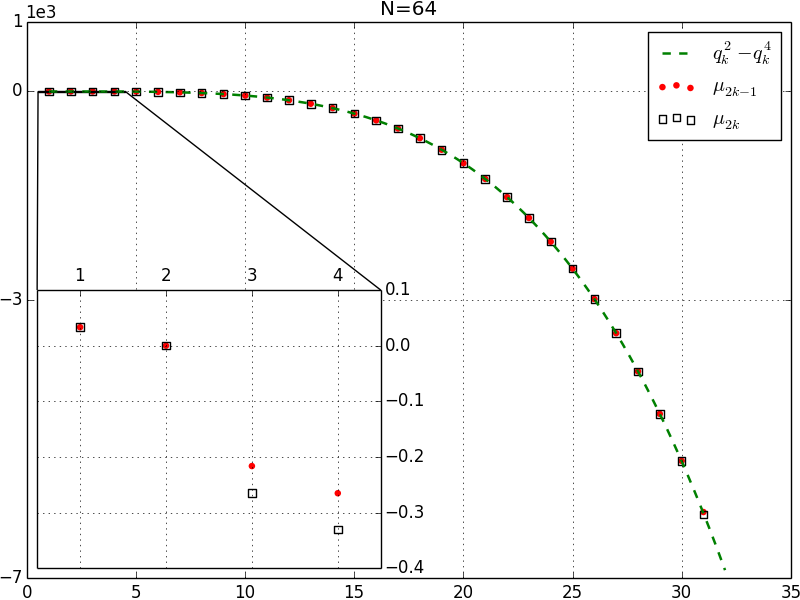
\includegraphics[width=0.7\textwidth]{KSspectrum}
    \end{figure}
\end{frame}

\subsection{Second stage: eigenvector algorithm}

\note{
  Given PRSF:

  \[
  \ps{\jMps}{k}=Q_{k}\ps{R}{k}Q_{k}^\top \,, \quad
  \ps{R}{k}=R_{k}R_{k-1}\cdots R_{1}R_{m}\cdots R_{k+1}
  \,.
  \]
  How to calculate the eigenvectors of $\ps{R}{k}$ ?


  Two candidates:
  \begin{itemize}
  \item {\color{green} Iteration method} \\
    \textbf{Prerequisite}: eigenvalues are ordered ascend/descend. Choose
    the latter which is outcome of Simultaneous iteration.

    \textbf{Basic idea}: power iteration.


  \item {\color{green} Reordering method}

    \textbf{Observation}: the first eigenvector of $\ps{R}{k}$ is
    $\jEigvec[1]=(1,0,\cdots,0)^\top $ if it is real.

    \textbf{Basic idea}: reorder the elements on the diagonal
    of $\ps{R}{k}$.

  \end{itemize}
}



\begin{frame}
  \frametitle{Candidate 1 : iteration method}

  Two case:
  \begin{itemize}
  \item \textbf{Real eigenvectors}:

    $i_{th}$ eigenvector :
    $\jEigvec[i]=(a_{1},a_{2},\cdots,a_{i},0,\cdots, 0)^\top $.

    \vspace{1em}
    Let $x=(b_{1},b_{2},\cdots,b_{i},0,\cdots, 0)^\top
    =\sum_{j=1}^{i}\alpha_{j}\jEigvec[j]$.
    \[
    (\ps{R}{k})^{-\ell}x
    \Rightarrow
    \lim_{\ell\to \infty} \frac{(\ps{R}{k})^{-\ell}x}{||\cdot||}=\jEigvec[i]
    \,.
    \]

    \pause

  \item \textbf{Complex eigenvector pairs}:

    The subspace $[x_1, x_2]$ converges to $X=[X_{1},X_{2}]$, and
    \[
      (\ps{R}{k})^{-1}X=X^{'}=XC
      \,,
      \label{eq:similar}
    \]
    $C$ eigenvectors : $\jEigvec[C]$ and $(\jEigvec[C])^{*}$.

    \[
    [\jEigvec[i],(\jEigvec[i])^{*}]=X[\jEigvec[C],(\jEigvec[C])^{*}]
    \]
  \end{itemize}

  \note[item]<1>{
    $(\ps{R}{k})^{-1}=R_{k+1}^{-1}\cdots R_{m}^{-1}R_{1}^{-1}R_{2}^{-1}\cdots
    R_{k}^{-1}$ has the same eigenvectors as $\ps{R}{k}$, but inverse
    eigenvalues.
  }

  \note[item]<1>{
    The $i_{th}$ and $(i+1)_{th}$ eigenvectors of $\ps{R}{k}$ form a
    complex pair.

    Let
    \[
    x_{1,2}=(\sum_{j=1}^{i-1}\alpha^{(1,2)}_{j}\jEigvec[j])+
    \alpha^{(1,2)}_{i}\jEigvec[i]+
    (\alpha^{(1,2)}_{i}\jEigvec[i])^{*}
    \,,
    \]
  }

  \note[item]<1>{
    where $C$ is a $[2\!\times\! 2]$ matrix which has two complex conjugate
    eigenvectors $\jEigvec[C]$ and $(\jEigvec[C])^{*}$.
  }
\end{frame}

\begin{frame}
  \frametitle{Problem 1}

  \begin{exampleblock}{Problem with the power iteration }
    {\color{red} Low efficiency when eigenvalues cluster.
      $\eigRe[i]\approx \eigRe[i-1]$}

  \end{exampleblock}

  \vspace{1em}
  \pause

  Candidate acceleration:
  \begin{itemize}
  \item {\color{cyan} Inverse iteration}:

    need to solve $((\ps{R}{k})^{-1}-sI)y=x$

    \pause
  \item {\color{cyan} Shifted power iteration}:

    $(\ps{R}{k})^{-1}-sI$ has the same
    eigenvectors as $(\ps{R}{k})^{-1}$

  \end{itemize}



  \note[item]<1>{
    Assume the eigenvalues of $\ps{R}{k}$ are
    $|\ExpaEig_{1}|\geq |\ExpaEig_{2}| \geq\cdots\geq
    |\ExpaEig_{n}|$. Each $\ExpaEig_{i}=e^{\eigExp[i]}$ with
    $\eigExp[i]=\eigRe[i]+i\eigIm[i]\,, \eigIm \in [0,2\pi)$.
    Assume that $\eigRe[i]\approx
    \eigRe[i-1]$, so pure power iteration converges slowly for the $i_{th}$
    eigenvector $\jEigvec[i]$.
  }
  \note[item]<1>{
    Inverse iteration is cumbersome here because $\ps{R}{k}$ is a product
    of a sequence of matrices.
  }
  \note[item]<1>{
    We turn to the second choice.
  }
  \note[item]<1>{
    remember to explain the meaning of $\eigRe[i]$.
  }
\end{frame}

\begin{frame}
  \frametitle{Shifted power iteration}
  Two scenarios:
  \begin{itemize}

  \item  ($\ExpaEig_{i-1}$, $\jEigvec[i-1]$) is real.

    Take {\color{green} $e^{\eigExp[i-1]}(\ps{R}{k})^{-1} -I$}.

    \begin{equation}
      \label{eq:numshifted}
      N=\max_{j=1}^{i-2}\dfrac{\ln
        \left(r_{0}\left|\dfrac{e^{\eigExp[i-1]-\eigExp[i]}-1}
            {e^{\eigExp[i-1]-\eigExp[j]}-1}\right|\right)}{\mu_i - \mu_j}
      \,.
    \end{equation}

    \pause

  \item ($\ExpaEig_{i-1}$, $\jEigvec[i-1]$) is complex.

    power iteration takes form
    {\color{green}
      $
      (e^{\eigExp[i-1]}(\ps{R}{k})^{-1} -I)
      (e^{\eigExp[i-1]{}^{*}}(\ps{R}{k})^{-1} -I)
      $.
    }
    \begin{equation}
      \label{eq:numshifted2}
      N=\max_{j=1}^{i-3}\dfrac{\ln \left(r_{0} \left|\dfrac{\exp(2\eigRe[i-1]-
              2\eigExp[i])-2\cos\eigIm[i-1]\exp(\eigRe[i-1]-\eigExp[i])+1}
            {\exp(2\eigRe[i-1]-2\eigExp[j])-
              2\cos\eigIm[i-1]\exp(\eigRe[i-1]-\eigExp[j])+1}
          \right|\right)}{\mu_i -\mu_j}
      \,.
    \end{equation}
  \end{itemize}

  \note[item]<1>{
    To annihilate both $a_{i-1}\jEigvec[i-1]$ and
    $(a_{i-1}\jEigvec[i-1])^{*}$,
  }

  \note[item]<1>{
    Explain the meaning of $N$.
  }
\end{frame}

\begin{frame}
  \frametitle{Problem 2}
  \begin{figure}[h]
    \centering
    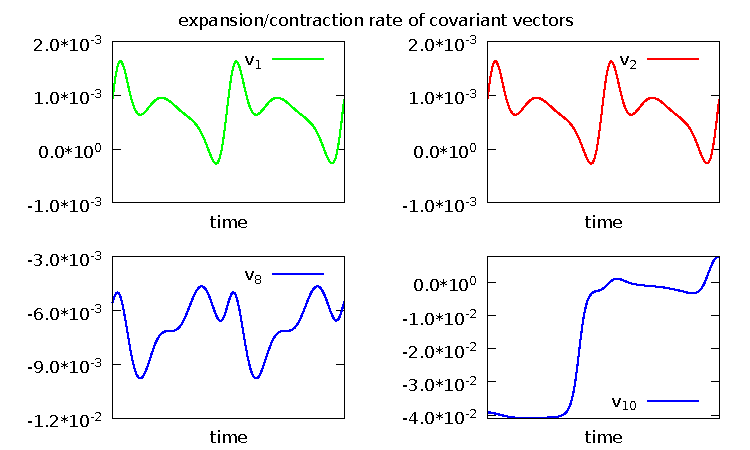
\includegraphics[width=0.9\textwidth]{ppo1rate}
  \end{figure}
  \note[item]<1>{
    The local expansion rate is obtained by evolving the Floquet vectors
    by the dynamics in the tangent space.
  }
  \note[item]<1>{
    The cyclic rotations of the sequence product.
    The only solution is use the eigenvectors at nearby points as the initial
    guess for the power iteration.
  }
\end{frame}


\begin{frame}
  \frametitle{Candidate 2 : Reordering algorithm~\cite{GranatK06}}

  Partition $R_{i}$ as
  \[
  R_{i}=
  \left[
    \begin{array}{c|cc|c}
      R^{00}_{i} & * & *& * \\ \hline
      0 & R^{11}_{i} & R^{12}_{i} & * \\
      0 & 0 & R^{22}_{i} & * \\ \hline
      0 & 0 & 0 & R^{33}_{i}
    \end{array}
  \right]
  \,,
  \]

  \textbf{Goal}: {\color{red} exchange $R^{11}_{i}$ with $R^{22}_{i}$}.

  \note[item]<1>{
    Be careful here. I must mention that this is not new, it is documented
    in the literature, but I use this technique here to show that it can
    help get eigenvectors.
  }
  \note[item]<1>{
    Remember to tell the audience the dimension of each block.
  }

  \note[item]<1>{
    Limitation of iteration method:
    \begin{itemize}
    \item need to combine pure\&shifted power iteration
      when eigenvalues cluster.
    \item Only can obtain eigenvectors for a specific $\ps{R}{k}$ at one
      time. Need iteration for other $k$.
    \end{itemize}
     Can we obtain eigenvectors for all $\ps{R}{k}$ at once?
     Method : Change the diagonal structure of each $R_i$.
  }
\end{frame}

\begin{frame}[allowframebreaks]
  \frametitle{Candidate 2 : Reodering algorithm}

  Try to construct  $\hat{S_{i}},\:i=0,1,2,\cdots,m$ with
  $\hat{S_{0}}=\hat{S_{m}}$
  \[
  \hat{S_{i}}=
  \left[
    \begin{array}{c|c|c}
      I_{p_{0}} & 0 & 0  \\ \hline
      0 & S_{i} & 0 \\ \hline
      0 & 0 & I_{p_{3}}
    \end{array}
  \right]
  \,,
  \quad
  S_{i}=
  \left[
    \begin{array}{c c}
      X_{i} & I_{p_{1}} \\
      I_{p_{2}} & 0
    \end{array}
  \right]
  \,.
  \]
  such that:
  \[
  \hat{S}_{i}^{-1}R_{i}\hat{S}_{i-1}=\tilde{R}_{i}=
  \left[
    \begin{array}{c|cc|c}
      R^{00}_{i} & * & *& * \\ \hline
      0 & R^{22}_{i} & 0 & * \\
      0 & 0 & R^{11}_{i} & * \\ \hline
      0 & 0 & 0 & R^{33}_{i}
    \end{array}
  \right]
  \,.
  \]
  That is
 {\color{red} \textbf{periodic Sylvester equation}}:
  \begin{equation}
    \label{eq:xdpse}
    R^{11}_{i}X_{i-1}-X_{i}R^{22}_{i}=-R^{12}_{i}
    \,,\quad i=0,1,2,\cdots,m
    \,.
  \end{equation}

  \note[item]<1>{
    Only consider {\color{red} two cases}: $R^{22}_i$ has dimension $[1\!\times\! 1]$
    or $[2\!\times\! 2]$.
  }

  \note[item]<1>{
    Sylvester [sil'vest\textipa{@}]
  }

  \begin{itemize}
  \item Real eigenvectors.

    \begin{equation}
      \label{eq:xdpsereal}
      \resizebox{\linewidth}{!}{%
        $
      \begin{bmatrix}
        R^{11}_{1} & -R^{22}_{1}I_{p_{1}} &  & \\[1em]
        & R^{11}_{2} & -R^{22}_{2}I_{p_{1}} &  &\\[1em]
        &  & R^{11}_{3} & -R^{22}_{3}I_{p_{1}} &  &\\[1em]
        & & & \ddots &\cdots & \\[1em]
        -R^{22}_{m}I_{p_{1}} & & & & R^{11}_{m}
      \end{bmatrix}
      \begin{bmatrix}
        X_{0} \\[1em]
        X_{1}  \\[1em]
        X_{2}  \\[1em]
        \cdots \\[1em]
        X_{m-1}
      \end{bmatrix}
      =
      \begin{bmatrix}
        -R^{12}_{1} \\[1em]
        -R^{12}_{2} \\[1em]
        -R^{12}_{3} \\[1em]
        \cdots \\[1em]
        -R^{12}_{m}
      \end{bmatrix} $%
    }
    \,.
    \end{equation}
     Defining
     $\mathbf{\tilde{R}}_{0}=\tilde{R}_{m}\tilde{R}_{m-1}\cdots
     \tilde{R}_{1}$, we get
     $\hat{S}_{m}^{-1}\ps{R}{0}\hat{S}_{m}=\mathbf{\tilde{R}}_{0}$.

     First eigenvector of $\mathbf{\tilde{R}}_{0}$ is
     $\tilde{e}=(1,0,\cdots , 0)^\top $, so
     \[
     \jEigvec[p_{1}+1]=\hat{S}_{m}\tilde{e}
     = \left[X_{0}^\top , 1, 0, 0, \cdots, 0 \right]^\top
     \,.
     \]
     Because of {\color{red} cyclic rotation}, for $\ps{R}{k}$ :
     $\jEigvec[p_{1}+1]=[X_{k}^\top,1,0,\cdots,0]^\top $.

     \note[item]<1>{
       Therefore, by solving one equation, we get eigenvectors for all
       $\ps{R}{k}$.
     }

   \item Complex conjugate eigenvector pairs.

       $R^{22}_i$ has dimension $[2\!\times\! 2]$.
       \begin{equation}
         \label{eq:xdpsdcomplex}
         \resizebox{\linewidth}{!}{%
           $
           \setlength{\arraycolsep}{3pt}
           \begin{bmatrix}
             I_{2}\otimes R^{11}_{1} & -(R^{22}_{1})^\top \otimes I_{p_{1}} &  & \\[1em]
             & I_{2}\otimes R^{11}_{2} & -(R^{22}_{2})^\top  \otimes I_{p_{1}} &  &\\[1em]
             &  & I_{2}\otimes R^{11}_{3} & -(R^{22}_{3})^\top \otimes I_{p_{1}} &  &\\[1em]
             & & & \ddots &\cdots & \\[1em]
             -(R^{22}_{m})^\top \otimes I_{p_{1}} & & & & I_{2}\otimes R^{11}_{m}
           \end{bmatrix}
           \begin{bmatrix}
             v(X_{0}) \\[1em]
             v(X_{1})  \\[1em]
             v(X_{2})  \\[1em]
             \cdots \\[1em]
             v(X_{m-1})
           \end{bmatrix}
           =
           \begin{bmatrix}
             -v(R^{12}_{1}) \\[1em]
             -v(R^{12}_{2}) \\[1em]
             -v(R^{12}_{3}) \\[1em]
             \cdots \\[1em]
             -v(R^{12}_{m})
           \end{bmatrix} $%
         }
         \,.
       \end{equation}
       Let $R^{22}=R^{22}_{m}R^{22}_{m-1}\cdots R^{22}_{1}$ with its two complex
       eigenvectors $v$ and $v^{*}$ of size $[2\!\times\! 1]$.

       Then the first two eigenvectors of  $\mathbf{\tilde{R}}_{0}$ are
       $\tilde{e}_{1}=(v^\top,0,0,\cdots,0)^\top $ and
       $\tilde{e}_{2}=(\tilde{e}_{1})^{*}$.

       The two corresponding eigenvectors of $\ps{R}{0}$ are
       \[
       \left[\jEigvec[p_{1}+1],\jEigvec[p_{1}+2]\right]
       =\hat{S}_{m}[\tilde{e}_{1},\tilde{e}_{2}]
       = \left[
         \begin{array}{c}
           X_{0} \\
           I_{2}    \\
           0 \quad 0\\
           0 \quad 0\\
           \vdots\\
           0 \quad 0
         \end{array}
       \right]
       [v,v^{*}]
       \,.
       \]

       Follow the same argument in the real case, we obtain complex conjugate
       eigenvectors for all $\ps{R}{k}$ by solving a single equation.

  \end{itemize}

\end{frame}

\subsection{Floquet vectors in \KSe}

\begin{frame}
  %\frametitle{Floquet vectors}
  \begin{figure}[h]
    \centering
    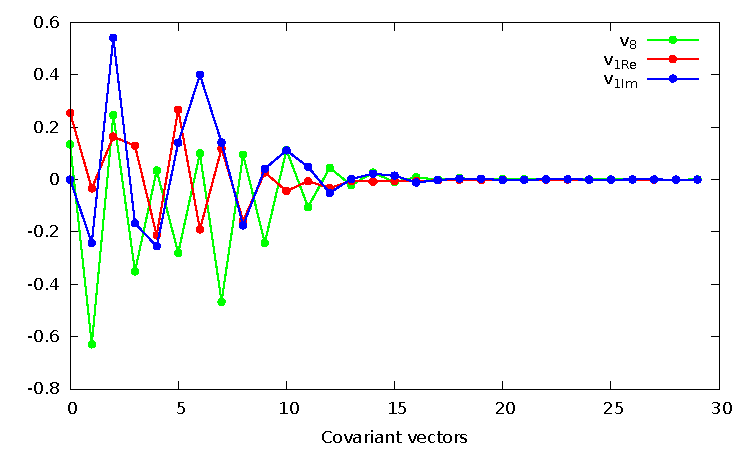
\includegraphics[width=0.7\textwidth, height=0.45\textheight]{ppo1ev_low}
  \end{figure}
  \begin{figure}[h]
    \centering
    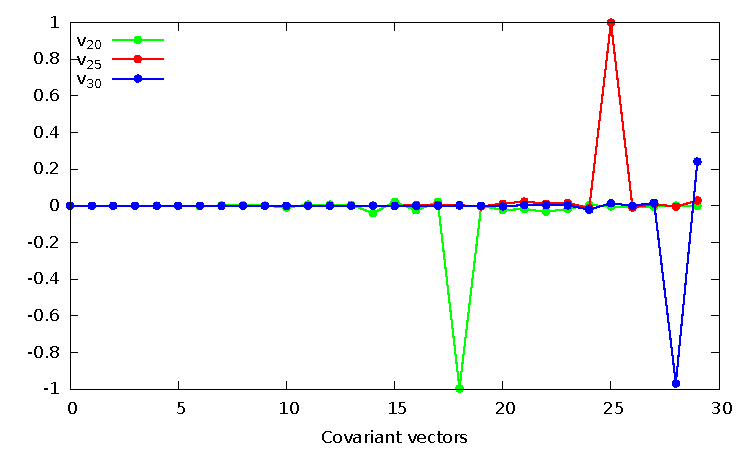
\includegraphics[width=0.7\textwidth, height=0.45\textheight]{ppo1ev_high}
  \end{figure}
\end{frame}

\begin{frame}
  \frametitle{Power spectrum}
  \begin{figure}[h]
    \centering
    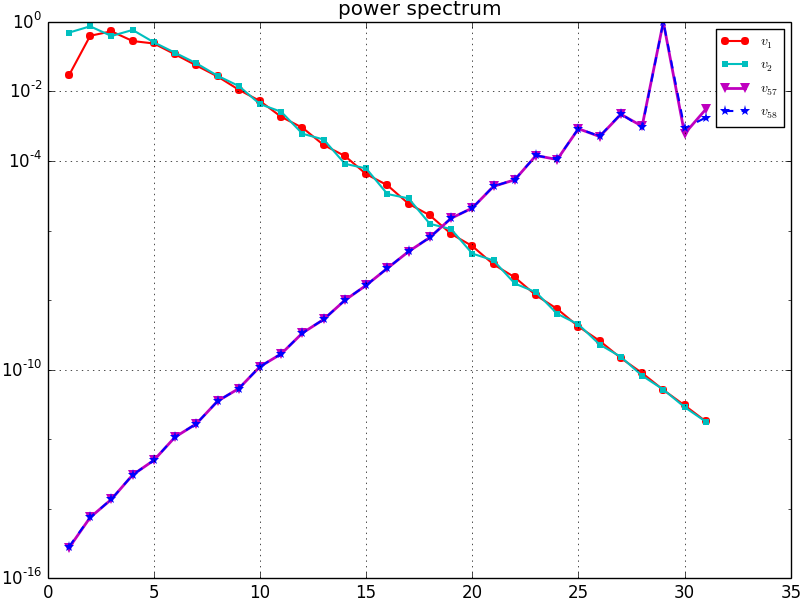
\includegraphics[width=0.7\textwidth]{KSpower}
  \end{figure}
\end{frame}

\begin{frame}
  \frametitle{Marginal Floquet vectors : \cycle{pp}}
    \begin{figure}[h]
    \centering
    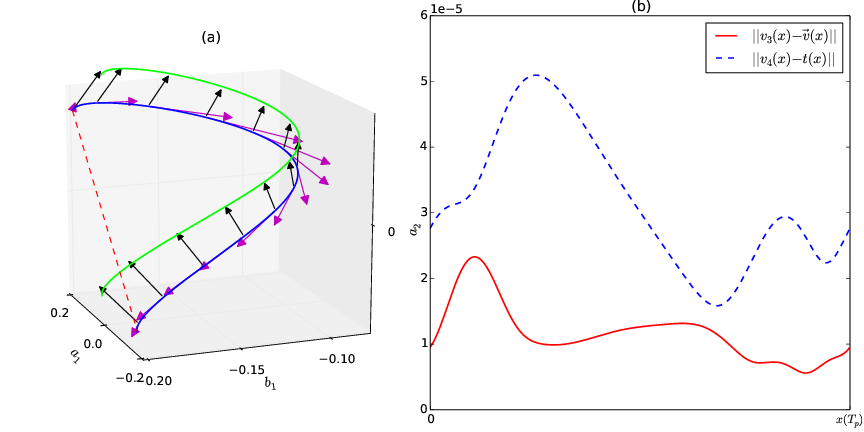
\includegraphics[width=1.0\textwidth]{ppo1vectfield2}
  \end{figure}
\end{frame}

\begin{frame}
  \frametitle{Marginal Floquet vectors : \cycle{rp}}
    \begin{figure}[h]
    \centering
    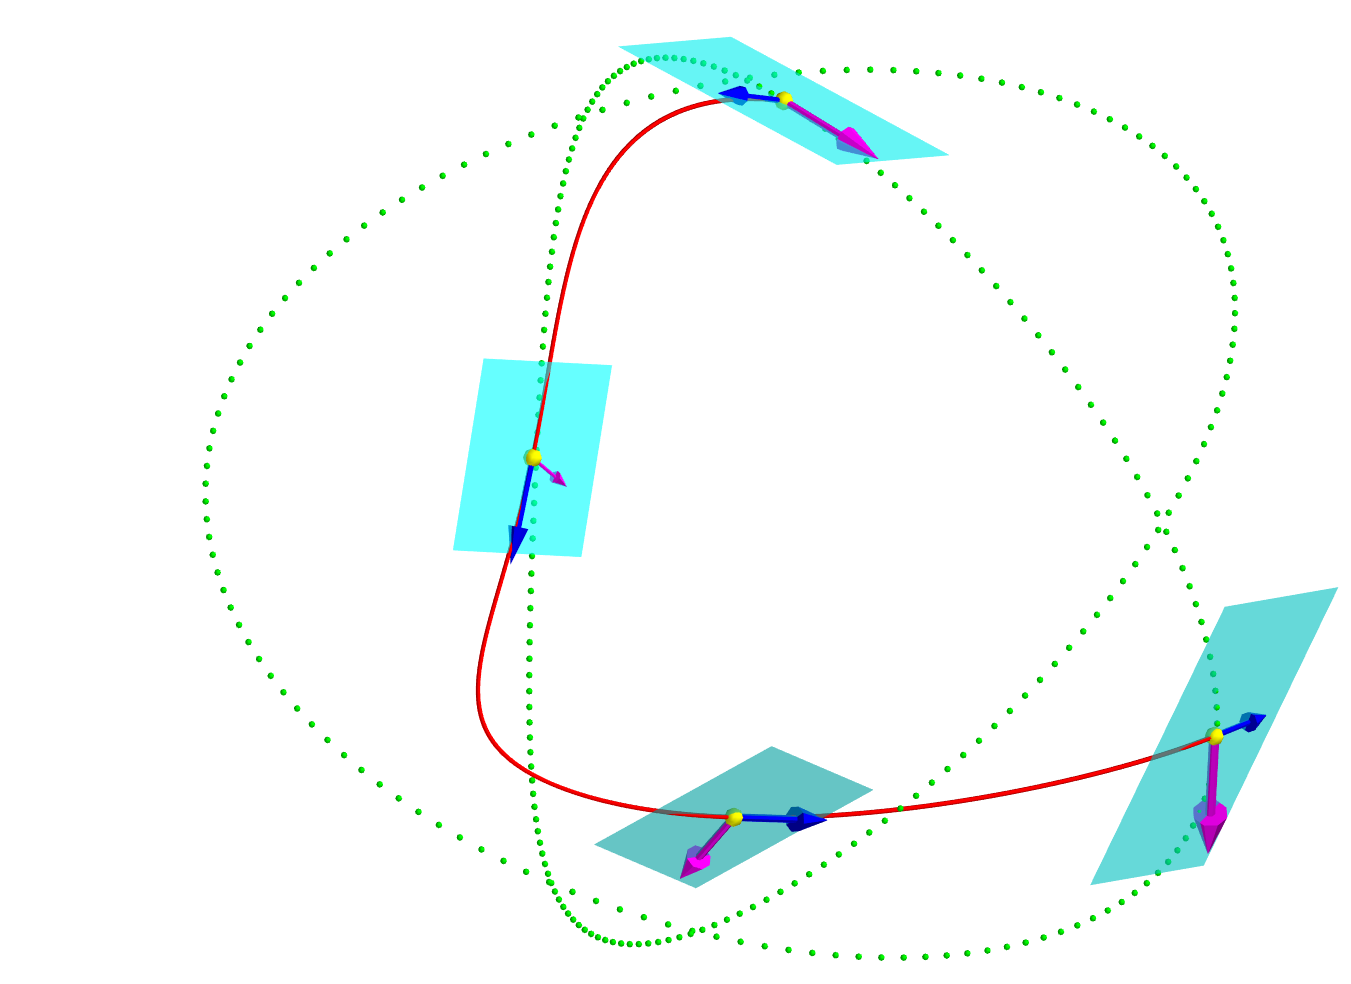
\includegraphics[width=0.9\textwidth]{rpo1_marginal3}
  \end{figure}
\end{frame}

\section{Computational effort}

\subsection{Stage 1}

\begin{frame}
  \frametitle{Periodic Schur decomposition vs Simultaneous iteration}
  \begin{block}{Periodic Schur decomposition}

    \begin{itemize}
    \item {\color{cyan} Hessenberg-triangular form} :

      $O(mn)$ Householder reflections
      with each reflection is $O(n^{2})$.
    \item {\color{cyan} Periodic QR} : for each iteration

      $O(mn)$
      Givens rotations with overall computational cost of $O(mn^{2})$
    \end{itemize}
  \end{block}

  \pause

  \begin{block}{  Simultaneous iteration: for each iteration}
    $m$ {\color{cyan} QR decomposition}
    $O(mn^{3})$ and $m$ {\color{cyan} matrix-matrix multiplication}
    $O(mn^{3})$ in each iteration.

    Total computational cost : $O(mn^{3})$
  \end{block}

  \pause

  Convergence  rate for both methods:
  $|\ExpaEig_{i}|/|\ExpaEig_{i+1}|$  without shift.

  Approximate ratio of cost : $\approx O(mn^3)/O(mn^2) = O(n)$

\end{frame}

\subsection{Stage 2}
\begin{frame}
  \frametitle{Power iteration vs Reordering}

  \begin{block}{Power iteration: for each iteration}
     $O(mi^{2})$ for the $i_{th}$ eigenvector
  \end{block}

  \pause

  \begin{block}{Reordering}
    Depend on an effective method to solve \textbf{\pse} \eqref{eq:xdpse}.
    \vspace{0em}

    For
    example, {\color{cyan} Gaussian  elimination with partial pivoting} (GEPP)
    has computational cost of $O(mn^{2})$.
  \end{block}

  \pause

  However,  the reordering method is {\color{red} not iterative} and
  it gives all the eigenvectors {\color{red} simultaneously}.
\end{frame}

\begin{frame}
  \frametitle{Floquet exponents}

  \begin{table}[h]
    \footnotesize
    \centering
    \caption{
    Eigenvalues
      {\color{red} $ |\ExpaEig_i|= \exp(\period{}\,\eigRe[i])$}
    of the Jacobian matrices for
      orbits $\cycle{pp}$ and $\cycle{rp}$, all computed to the machine
      precision, vary from $O(1)$ to
      $O(10^{-145})$!
    }
    \label{tab:floquet_ppo1}
    \begin{tabu}{l l c|[1pt]l l c}
      % \tabucline[1pt]{-}
      \multicolumn{3}{c|[1pt]}{$\cycle{pp}$} & \multicolumn{3}{c}{$\cycle{rp}$}\\
      $i$ & ~~~~~$\eigRe[i]$  & $\theta_{i}$  & $i$ & ~~~~~$\eigRe[i]$ & $\theta_{i}$  \\
      \tabucline[1pt]{-}
      1,2 & ~0.033209  &    $\pm$2.0079  &  1 &    ~0.32791  &              \\
      3 & -2.0317e-14  &                 &  2 &   ~5.0352e-09  &              \\
      4 & -2.4267e-09  &    -1           &  3 &  -1.2399e-08  &              \\
      5 &  -0.21637    &                 &  4 &     -0.13214  &        -1    \\
      6,7 &  -0.26524  &   $\pm$2.6205   &  5,6 &   -0.28597  & $\pm$2.7724  \\
      8 &  -0.33073    &    -1           &  7 &     -0.36242  &              \\
      9 &  -1.9605    &                  &  8 &      -0.32821  &      -1     \\
      10 & -1.9676    &    -1            &  9,10 &   -1.9617  &  $\pm$2.2411 \\
      $\cdots$ &  $\cdots$    & $\cdots$ & $\cdots$ & $\cdots$ & $\cdots$   \\
      27 &  -239.52   &                 & $\cdots$ & $\cdots$ &  $\cdots$   \\
      28 &  -239.22    &    -1           &  27,28 &    -239.41& $\pm$0.88159 \\
      29 & -307.47     &    -1           &  29 &      -313.98 &              \\
      30 & -332.74     &                 &  30 &      -323.41 &              \\
      \tabucline[1pt]{-}
    \end{tabu}
  \end{table}

\end{frame}

\usebackgroundtemplate
{
  
\includegraphics[width=\paperwidth,height=\paperheight]{./figs/lastpage.jpg}%
}
\begin{frame}

  \centering{ \huge Thank you for the time !}

  \vspace{2em}

  \centering{ \huge Any questions ?}
\end{frame}


\usebackgroundtemplate
{
  
\includegraphics[width=\paperwidth,height=\paperheight]{./figs/background.jpg}%
}

\begin{frame}[allowframebreaks]
  \frametitle{References}
  \scriptsize{\bibliographystyle{acm}}
  \bibliography{../../bibtex/siminos}
\end{frame}


\begin{frame}[allowframebreaks]
  \frametitle{Backup}
  Steps:
  \begin{enumerate}
  \item An arbitrary initial vector
    $\tilde{q}_{1}=\sum_{i=1}^{n}\alpha^{(1)}_{i}v_{i}$
    \[
    \lim_{\ell\to \infty }\frac{(\ps{\jMps}{0})^{\ell}\tilde{q}_{1}}{||\cdot||}
    \to q_{1}=v_{1}
    \,.
    \]

  \item After got $q_1$, chose arbitrary $\tilde{q}_{2}$ orthogonal to
    subspace $\langle q_{1} \rangle$
    \[
    \tilde{q}_{2}= \sum_{i=2}^{n}\alpha^{(2)}_{i}[v_{i}-(q_{1}^\top
    v_{i})q_{1}]
    \,.
    \]
    Apply power
    iteration of $\ps{\jMps}{0}$ followed by orthonormalization:
    \begin{align*}
      \ps{\jMps}{0}\tilde{q}_{2}= &\sum_{i=2}^{n}\alpha^{(2)}_{i}
      [\ExpaEig_{i}v_{i}-\ExpaEig_{1}(q_{1}^\top v_{i})v_{1}] \\
      = & \sum_{i=2}^{n}\alpha^{(2)}_{i}\ExpaEig_{i}[v_{i}-
      (q_{1}^\top v_{i})v_{1}]+\sum_{i=2}^{n}\alpha^{(2)}_{i}
      (\ExpaEig_{i}-\ExpaEig_{1})(q_{1}^\top v_{i})v_{1}
      \,.
    \end{align*}
    The second term disappears after performing orthonormalization.
    Finally, we get $q_{2}=v_{2}-(q_{1}^\top v_{2})v_{1}$.


  \item Suppose $\tilde{q}_{j-1}$ converges to
    \[
    q_{j-1}=v_{j-1}-\sum_{s=1}^{j-2}(q_{s}^\top v_{j-1})q_{s}
    \,.
    \]
    Also note $\langle v_{1},v_{2},\cdots,v_{j-1}\rangle=\langle
    q_{1},q_{2},\cdots,q_{j-1}\rangle$. \\
    Then Choose an arbitrary vector
    $\tilde{q}_{j}$ perpendicular to subspace $\langle
    v_{1},v_{2},\cdots,v_{j-1}\rangle$:
    \[
    \tilde{q}_{j}=\sum_{i=j}^{n}\alpha_{i}^{(j)}[v_{i}-\sum_{s=1}^{j-1}
    (q^\top _{s}v_{i})q_{s}]
    \,.
    \]
    After one iteration:
    \begin{align*}
      \ps{\jMps}{0}\tilde{q}_{j}
      = & \sum_{i=j}^{n}\alpha^{(j)}_{i}\ExpaEig_{i}
      \left[v_{i}-\sum_{s=1}^{j-1}(q_{s}^\top v_{i})q_{s}\right]
      +
      \sum_{i=j}^{n}\alpha^{(j)}_{i}\sum_{s=1}^{j-1}
      (\ExpaEig_{i}-\ExpaEig_{s})(q_{s}^\top v_{i})q_{s}
      \,.
    \end{align*}
    Second term disappears after performing orthonormalization to
    $\langle  v_{1},v_{2},\cdots,v_{j-1}\rangle$.
    So,
    \[
    q_{j}=v_{j}-\sum_{s=1}^{j-1}(q_{s}^\top v_{j})q_{s}
    \,.
    \]
  \end{enumerate}

  %%%%%%%%%%%%%%%%%%%%%%%%%%%%%%%%%%%%%%%%%%%%
  Let $Q_{0}=[q_{1},q_{2},\cdots ,q_{n}]$; then
  $\ps{\jMps}{0}Q_{0}=Q_{0}\ps{R}{0}$.
  \begin{algorithm}[H]
    \caption{Simultaneous Iteration}
    \label{ag:simuliter}
    \begin{algorithmic}
      \State $\tilde{Q}_{0}$: an arbitrary orthogonal $n\times n$ matrix
      \For{$i=1,2,\cdots$}
      \For{$s=1:m$}
      \State $J_{s}\tilde{Q}_{s-1}=\tilde{Q}_{s}\tilde{R}_{s}$
      \EndFor
      \State $\tilde{Q}_{0}=\tilde{Q}_{m}$
      \EndFor
    \end{algorithmic}
  \end{algorithm}

  %%%%%%%%%%%%%%%%%%%%%%%%%%%%%%
  \begin{itemize}

  \item  ($\ExpaEig_{i-1}$, $\jEigvec[i-1]$) is real.
    Let
    \[
    x=(\sum_{j=1}^{i-2}\alpha_{j}\jEigvec[j])
    +      \alpha_{i-1}\jEigvec[i-1]+\alpha_{i}\jEigvec[i]+
    (\alpha_{i}\jEigvec[i])^{*}
    \,.
    \]
    a general vector with first $i$ elements nonzero regardless
    $\jEigvec[i]$ real or complex.

    \bea
    \left(e^{\eigExp[i-1]}(\ps{R}{k})^{-1} -I\right)x
    &=&
    \sum_{j=1}^{i-2}\alpha_{j}(e^{\eigExp[i-1]-\eigExp[j]}-1)\jEigvec[j]
    \ceq
    +\;
    \alpha_{i}(e^{\eigExp[i-1]-\eigExp[i]}-1)\,\jEigvec[i]
    +
    \alpha_{i}^{*}(e^{\eigExp[i-1]-\eigExp[i]^{*}}-1)\,\jEigvec[i]^{*}
    \,.
    \nnu
    \eea

    \[
    \left|
      e^{(\eigExp[i]-\eigExp[j])N}\cdot \frac{e^{\eigExp[i-1]-\eigExp[j]}-1}
      {e^{\eigExp[i-1]-\eigExp[i]}-1}
    \right|=r_{0}
    \,,
    \]

    \begin{equation}
      N=\max_{j=1}^{i-2}\dfrac{\ln
        \left(r_{0}\left|\dfrac{e^{\eigExp[i-1]-\eigExp[i]}-1}
            {e^{\eigExp[i-1]-\eigExp[j]}-1}\right|\right)}{\mu_i - \mu_j}
      \,.
    \end{equation}

  \item ($\ExpaEig_{i-1}$, $\jEigvec[i-1]$) is complex.

    To annihilate both $a_{i-1}\jEigvec[i-1]$ and
    $(a_{i-1}\jEigvec[i-1])^{*}$, power iteration takes form
    $
    (e^{\eigExp[i-1]}(\ps{R}{k})^{-1} -I)
    (e^{\eigExp[i-1]{}^{*}}(\ps{R}{k})^{-1} -I)
    $.

    \begin{equation}
      N=\max_{j=1}^{i-3}\dfrac{\ln \left(r_{0} \left|\dfrac{\exp(2\eigRe[i-1]-
              2\eigExp[i])-2\cos\eigIm[i-1]\exp(\eigRe[i-1]-\eigExp[i])+1}
            {\exp(2\eigRe[i-1]-2\eigExp[j])-
              2\cos\eigIm[i-1]\exp(\eigRe[i-1]-\eigExp[j])+1}
          \right|\right)}{\mu_i -\mu_j}
      \,.
    \end{equation}
  \end{itemize}

%%%%%%%%%%%%%%%%%%%%%%%%%%%%%%%%%%%%%%%%

  \[
  a_{k}(t)=\frac{1}{N}\sum_{n=0}^{N-1}u(x_{n},t)e^{-iq_{k}x_{n}}
  \,,\quad
  u(x_{n},t)=  \sum_{k=-N/2+1}^{N/2} a_{k}(t)e^{iq_{k}x_{n}}
  \]

\end{frame}



\end{document}
